\documentclass{article}
\usepackage{amsmath}
\usepackage{tikz}
\usetikzlibrary{arrows}

\begin{document}
	%inkscape -l plot.svg plot.pdf
	\thispagestyle{empty}
	\begin{figure}
	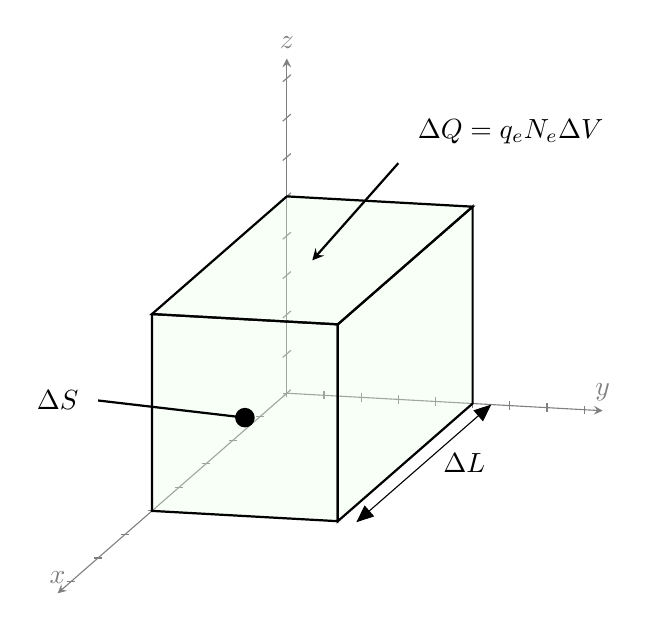
\begin{tikzpicture}[x=0.5cm,y=0.5cm,z=0.3cm,>=stealth, rotate around x=-90, rotate around y=-0, rotate around z=5]
		% The axes
		\draw[color=gray,->] (xyz cs:x=0) -- (xyz cs:x=8.5) node[above] {$y$};
		\draw[color=gray,->] (xyz cs:y=0) -- (xyz cs:y=8.5) node[above] {$x$};
		\draw[color=gray,->] (xyz cs:z=0) -- (xyz cs:z=8.5) node[above] {$z$};
		
		% The thin ticks
		\foreach \coo in {0,1,...,8}
		{
			\draw[color=gray] (\coo,-1.5pt) -- (\coo,1.5pt);
			\draw[color=gray] (-1.5pt,\coo) -- (1.5pt,\coo);
			\draw[color=gray] (xyz cs:y=-0.15pt,z=\coo) -- (xyz cs:y=0.15pt,z=\coo);
		}
		\coordinate (S) at (2.5,5,2.5);
		\coordinate (S0) at (0,7,4);
		\coordinate (L) at (5.5,2.5,0);
		\coordinate (Q) at (2.5,2.5,5);
		\coordinate (Q0) at (3,0,6);
		\coordinate (ooo) at (0,0,0);
		\coordinate (xoo) at (5,0,0);
		\coordinate (xyo) at (5,5,0);
		\coordinate (oyo) at (0,5,0);
		\coordinate (xoz) at (5,0,5);
		\coordinate (xyz) at (5,5,5);
		\coordinate (ooz) at (0,0,5);
		\coordinate (oyz) at (0,5,5);
		
		\coordinate (x2yo) at (5,2,0);
		\coordinate (o2yo) at (0,2,0);
		\coordinate (x2yz) at (5,2,5);
		\coordinate (o2yz) at (0,2,5);
		\coordinate (x7yo) at (5,7,0);
		\coordinate (o7yo) at (0,7,0);
		\coordinate (x7yz) at (5,7,5);
		\coordinate (o7yz) at (0,7,5);

		
		\fill[color=green!10,thick,fill opacity=0.3,draw=black] (oyo) -- (oyz) -- (xyz) -- (xyo) -- cycle;
		\fill[color=green!10,thick,fill opacity=0.3,draw=black] (xyo) -- (xyz) -- (xoz) -- (xoo) -- cycle;
		\fill[color=green!10,thick,fill opacity=0.3,draw=black] (oyz) -- (ooz) -- (xoz) -- (xyz) -- cycle;
		\draw[>=triangle 45, <->] (5.5,0) -- (5.5,5);
		
		\node[fill,circle,inner sep=2.5pt] at (S) {};
		\node[label={right:$\Delta L$}] at (L) {};
		\draw[thick] (S0) -- (S);
		\node[label={left:$\Delta S$}] at (S0) {};
		\draw[thick,->] (Q0) -- (Q);
		%\node[label={right:$\Delta Q = \rho_v \Delta V$}] at (Q0) {};
		\node[label={above right:$\Delta Q = q_e  N_e \Delta V$}] at (Q0) {};
	\end{tikzpicture}
	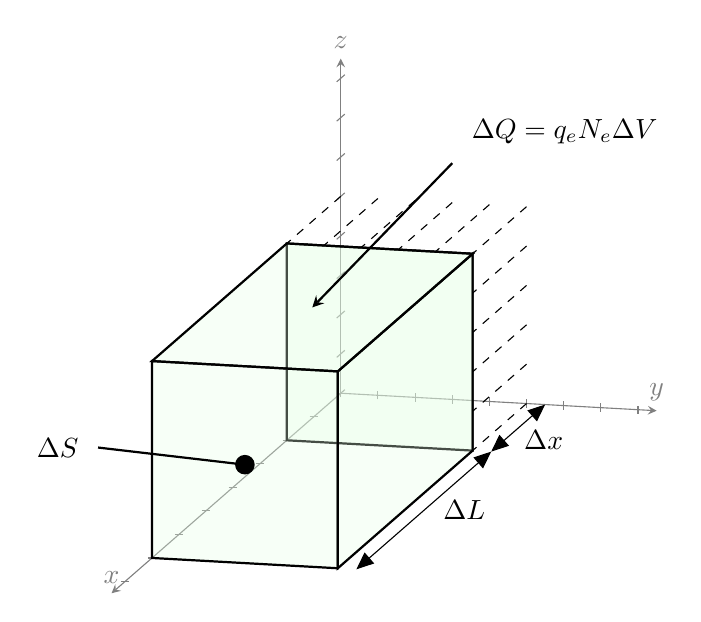
\begin{tikzpicture}[x=0.5cm,y=0.5cm,z=0.3cm,>=stealth, rotate around x=-90, rotate around y=-0, rotate around z=5]
	% The axes
	\draw[color=gray,->] (xyz cs:x=0) -- (xyz cs:x=8.5) node[above] {$y$};
	\draw[color=gray,->] (xyz cs:y=0) -- (xyz cs:y=8.5) node[above] {$x$};
	\draw[color=gray,->] (xyz cs:z=0) -- (xyz cs:z=8.5) node[above] {$z$};
	
	% The thin ticks
	\foreach \coo in {0,1,...,8}
	{
		\draw[color=gray] (\coo,-1.5pt) -- (\coo,1.5pt);
		\draw[color=gray] (-1.5pt,\coo) -- (1.5pt,\coo);
		\draw[color=gray] (xyz cs:y=-0.15pt,z=\coo) -- (xyz cs:y=0.15pt,z=\coo);
	}
	\coordinate (S) at (2.5,7,2.5);
	\coordinate (S0) at (0,9,4);
	\coordinate (L) at (5.5,4.5,0);
	\coordinate (Q) at (2.5,4.5,5);
	\coordinate (Q0) at (3,0,6);
	\coordinate (dy) at (5.5,1.5,0);
	
	
	\coordinate (x2yo) at (5,2,0);
	\coordinate (o2yo) at (0,2,0);
	\coordinate (x2yz) at (5,2,5);
	\coordinate (o2yz) at (0,2,5);
	\coordinate (x7yo) at (5,7,0);
	\coordinate (o7yo) at (0,7,0);
	\coordinate (x7yz) at (5,7,5);
	\coordinate (o7yz) at (0,7,5);
	
	
	\fill[color=green!10,thick,fill opacity=0.3,draw=black] (o2yo) -- (o2yz) -- (x2yz) -- (x2yo) -- cycle;
	\fill[color=green!10,thick,fill opacity=0.3,draw=black] (x7yo) -- (x7yz) -- (x2yz) -- (x2yo) -- cycle;
	\fill[color=green!10,thick,fill opacity=0.3,draw=black] (o7yz) -- (o2yz) -- (x2yz) -- (x7yz) -- cycle;
	\fill[color=green!10,thick,fill opacity=0.3,draw=black] (x7yz) -- (x7yo) -- (o7yo) -- (o7yz) -- cycle;
	\draw[>=triangle 45, <->] (5.5,2) -- (5.5,7);
	\draw[>=triangle 45, <->] (5.5,0) -- (5.5,2);
	
	\draw[dashed] (0,0,5) -- (0,2,5);
	\draw[dashed] (1,0,5) -- (1,2,5);
	\draw[dashed] (2,0,5) -- (2,2,5);
	\draw[dashed] (3,0,5) -- (3,2,5);
	\draw[dashed] (4,0,5) -- (4,2,5);
	\draw[dashed] (5,0,5) -- (5,2,5);
	\draw[dashed] (5,0,4) -- (5,2,4);
	\draw[dashed] (5,0,3) -- (5,2,3);
	\draw[dashed] (5,0,2) -- (5,2,2);
	\draw[dashed] (5,0,1) -- (5,2,1);
	\draw[dashed] (5,0,0) -- (5,2,0);
	
	\node[fill,circle,inner sep=2.5pt] at (S) {};
	\node[label={right:$\Delta L$}] at (L) {};
	\draw[thick] (S0) -- (S);
	\node[label={left:$\Delta S$}] at (S0) {};
	\draw[thick,->] (Q0) -- (Q);
	%\node[label={right:$\Delta Q = \rho_v \Delta V$}] at (Q0) {};
	\node[label={above right:$\Delta Q = q_e  N_e \Delta V$}] at (Q0) {};
	\node[label={right:$\Delta x$}] at (dy) {};
\end{tikzpicture}
	\end{figure}

\end{document}

